\section{Back propagation in CNN - an example}

In this question, we are going to do \textbf{back propagation} operation on a sequence of layers, shown below; and write the update rules (and update weights) for each of the weights using \textbf{gradient descent}.

\begin{center}
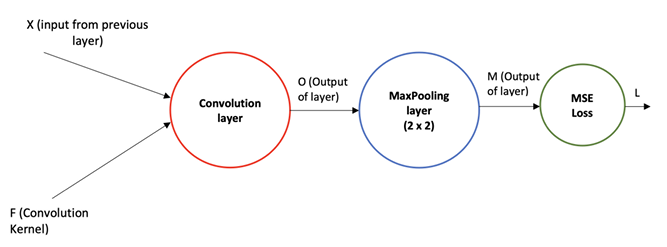
\includegraphics[width = 0.8\textwidth]{cnn_diagram.png} % Save your diagram image as cnn_diagram.png in the same directory as this .tex file.
\end{center}

Here, please write the update rules and then update weights corresponding to variables/matrices \(X, F, O, M\). The required information is provided below:

\[
X = \begin{bmatrix}
1 & 7 & -1 & -7 & 10 & 11 \\
2 & 8 & 0 & 0 & 12 & 13 \\
3 & 9 & 0 & 0 & 0 & 0 \\
4 & 10 & -4 & -10 & 0 & 0 \\
5 & 11 & -5 & -11 & 16 & 17 \\
6 & 12 & -6 & -12 & 14 & 15 \\
\end{bmatrix}
\]

\[
F = \begin{bmatrix}
1 & 0 & -1 \\
2 & 0 & -2 \\
1 & 0 & -1 \\
\end{bmatrix}
\]

\[
\mathcal{L} = \begin{bmatrix}
1 & 0 & 0 \\
0 & 1 & 0 \\
0 & 0 & 1 \\
\end{bmatrix}
\]

Where \(\mathcal{L}\) is the matrix to calculate MSE loss with.
\begin{qsolve}
    \begin{qsolve}[]
        we use the expressions of previous question:
        \[
        \frac{\partial L}{\partial F} = X * \frac{\partial L}{\partial O}
        \]
        first we calculate \(\frac{\partial L}{\partial O}\) and then we calculate \(\frac{\partial L}{\partial F}\) and update \(F\).
        for the calculation of \(\frac{\partial L}{\partial O}\) we need to calculate \(O\) and \(M\). so we have:
        \splitqsolve[\splitqsolve]
        \[
        O = X \overset{\text{valid}}{*} F = \begin{bmatrix}
        9 & 39 & -35 & -47 \\
        16 & 46 & -16 & -23 \\
        29 & 71 & -29 & -48 \\
        40 & 88 & -66 & -93 \\
        \end{bmatrix}
        \quad \xrightarrow{\text{max pooling}} \quad
        M = \begin{bmatrix}
        46 & 46 & -16 \\
        71 & 71 & -16 \\
        88 & 88 & -29 \\
        \end{bmatrix}
        \]

        \[
            L = \frac{1}{n} (\mathcal{L} - M)^T (\mathcal{L} - M) \Rightarrow \frac{\partial L}{\partial M} = \frac{2}{n} (M - \mathcal{L})
        \]

        \[
        \Rightarrow \frac{\partial L}{\partial M} =  \frac{2}{9} \begin{bmatrix}
        45 & 46 & -16 \\
        71 & 70 & -16 \\
        88 & 88 & -30 \\
        \end{bmatrix} = \begin{bmatrix}
        10 & 10.22 & -3.56 \\
        15.78 & 15.56 & -3.56 \\
        19.56 & 19.56 & -6.67 \\
        \end{bmatrix}
        \]
        now we calculate \(\frac{\partial L}{\partial O}\):\\
        Initializing \(\frac{\partial L}{\partial O}\) as a matrix of zeros with the same dimensions as \(O\).\\
        For each element in \(M\) (indexed by \(i, j\)), find the position \((k, l)\) in \(O\) that was the maximum in its pooling region.

        \[
        \Rightarrow \frac{\partial L}{\partial O_{k,l}} = \frac{\partial L}{\partial M_{i,j}}
        \]

        \[
        \Rightarrow \frac{\partial L}{\partial O} = \begin{bmatrix}
        0 & 0 & 0 & 0 \\
        0 & 20.22 & -7.12 & 0 \\
        0 & 31.34 & -6.67 & 0 \\
        0 & 39.12 & 0 & 0 \\
        \end{bmatrix}
        \]

        so we can calculate \(\frac{\partial L}{\partial F}\) and update \(F\):
        \[
        \frac{\partial L}{\partial F} = \begin{bmatrix}
        835.02 & -156.48 & -476.64 \\
        952.38 & -254.26 & -743.72 \\
        1078.21 & -327.73 & -1123.1 \\
        \end{bmatrix}
        \]

        \[
        F^{(\text{new})} = F^{(\text{old})} - \eta \frac{\partial L}{\partial F}
        \]   
        for example if we set \(\eta = 0.01\), we have:
        \[
        F^{(\text{new})} = \begin{bmatrix}
        1 & 0 & -1 \\
        2 & 0 & -2 \\
        1 & 0 & -1 \\
        \end{bmatrix} - 0.01 \begin{bmatrix}
        835.02 & -156.48 & -476.64 \\
        952.38 & -254.26 & -743.72 \\
        1078.21 & -327.73 & -1123.1 \\
        \end{bmatrix}
        = \begin{bmatrix}
            -7.35 & 1.56 & 3.77 \\
            -7.52 & 2.54 & 5.44 \\
            -9.78 & 3.28 & 10.23 \\
        \end{bmatrix}
        \]
    \end{qsolve}
\end{qsolve}